\documentclass[11pt]{beamer}
\usepackage{graphicx}
\graphicspath{ {./Images/} }
\setbeamertemplate{caption}[numbered]
\usepackage{caption}
\usepackage{float}
\usepackage{wasysym}
\usepackage{hyperref}
\usepackage{movie15}
%\usepackage[margin=1in]{geometry}
\usepackage{multirow}
\setbeamersize{text margin left=0.5cm,text margin right=0.5cm}
\usepackage{dirtytalk}
\usepackage{siunitx}
\usepackage{multicol}
\usepackage{listings}
\usepackage{color}
\usepackage{fancyvrb}
\usepackage{booktabs} % Allows the use of \toprule, \midrule and \bottomrule in tables
\definecolor{dkgreen}{rgb}{0,0.6,0}
\definecolor{gray}{rgb}{0.5,0.5,0.5}
\definecolor{mauve}{rgb}{0.58,0,0.82}
\lstset{
  language=Java,
  aboveskip=3mm,
  belowskip=3mm,
  showstringspaces=false,
  columns=flexible,
  basicstyle={\small\ttfamily},
  numbers=none,
  frame=single,
  numberstyle=\tiny\color{gray},
  keywordstyle=\color{blue},
  commentstyle=\color{dkgreen},
  stringstyle=\color{mauve},
  breaklines=true,
  breakatwhitespace=true,
  tabsize=3,
  fancyvrb=true,
}

% The following code is to pause within the align environment 
\makeatletter
\let\save@measuring@true\measuring@true
\def\measuring@true{%
  \save@measuring@true
  \def\beamer@sortzero##1{\beamer@ifnextcharospec{\beamer@sortzeroread{##1}}{}}%
  \def\beamer@sortzeroread##1<##2>{}%
  \def\beamer@finalnospec{}%
}
\makeatother

\mode<presentation> {
    \usetheme{Warsaw}
    % \setbeamertemplate{footline} % To remove the footer line in all slides uncomment this line
    \setbeamertemplate{footline}[page number] % To replace the footer line in all slides with a simple slide count uncomment this line
    % \setbeamertemplate{navigation symbols}{} % To remove the navigation symbols from the bottom of all slides uncomment this line    
    % \addtobeamertemplate{navigation symbols}{}{%
    %     \usebeamerfont{footline}%
    %     \usebeamercolor[fg]{footline}%
    %     \hspace{1em}%
    %     \insertframenumber/\inserttotalframenumber
        % }
    }
    
% macro for color
\definecolor{violet}{rgb}{0.54, 0.17, 0.89}
\newcommand{\red}[1]{\textcolor{red}{#1}}
\newcommand{\violet}[1]{\textcolor{violet}{#1}}
\newcommand{\green}[1]{\textcolor{green}{#1}}
\newcommand{\sol}{\textbf{Solution}: \pause \newline}

%----------------------------------------------------------------------------------------
%	TITLE PAGE
%----------------------------------------------------------------------------------------

\title[Chapter 05 Notes]{Math 130: Introduction to Programming \\ Chapter 05: Methods \\ Lecture Notes}

\author{Jesús R. Pérez Cuarenta \\
\href{mailto:jperezcuarenta@swccd.edu}{jperezcuarenta@swccd.edu}
}

\date{} % Date, can be changed to a custom date

\begin{document}
% 
% The Splash Slide(s) are not part of any section
% 
% \section{}
%%%%%%%%%%%%%%%%%%%%%%%%%%%%%%%%%%%%%%%%%%%%%%%%%%%%%%%%%%%%%%%%%%%%%% 

\begin{frame}
  \maketitle
\end{frame}

\begin{frame}
\frametitle{Overview}
    % \begin{multicols}{2}
    \tableofcontents
    % \end{multicols}
\end{frame}

\section{Introduction to Methods}
\subsection{Introduction}
\begin{frame}{Introduction to Methods}
    Methods can be used to break a complex program into small, manageable pieces. \\ 
    \vspace{1em} 
    A \textbf{void} method simply executes a group of statements and then terminates. \\ 
    \vspace{1em} 
    A value-returning method returns a value to the statement that called it.        
\end{frame}

\begin{frame}{Introduction to Methods}
    \noindent 
    \begin{figure}[H]
    \centering
    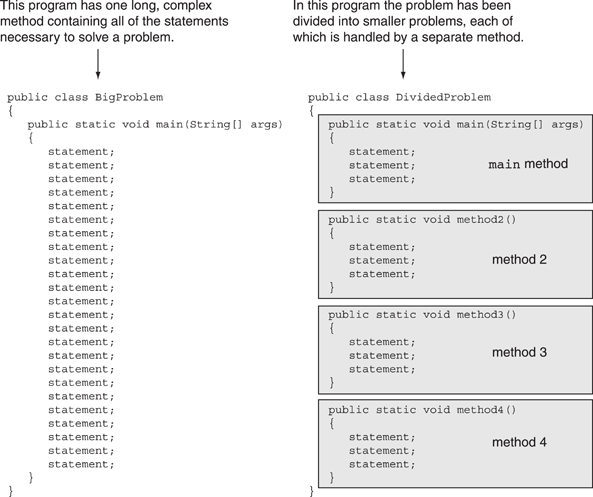
\includegraphics[scale=0.7]{Images/chapter05_motivation.png}
    \end{figure}
\end{frame}

\subsection{void Methods}
\begin{frame}[fragile]{void Methods}
    A \textbf{void} method simply performs a task and then terminates it.
    \begin{lstlisting}
int number = 7;
System.out.println(number); // void method
number = 0;
    \end{lstlisting}
    A value-returning method performs a task and sends a value back to the code that called in.
    \begin{lstlisting}
int number;
Random rand = new Random();
number = rand.nextInt(); // value-returning method
    \end{lstlisting}
\end{frame}

\begin{frame}[fragile]{Defining a void Method}
    To create a method you must write its definition, which consists of two general parts: header and a body.
    \begin{lstlisting}
public static void displayMessage() {
    System.out.println("Hello from the displayMessage method.");
    }
    \end{lstlisting}
\end{frame}

\begin{frame}{Defining a void Method}
\footnotesize
\begin{itemize}
    \item Method Modifiers \\
    The keyword \violet{\textbf{public}} means that the method is publicly available to code outside the class. The keyword \violet{\textbf{static}} means that the method belongs to a class.
    \item Return Type \\ 
    When we write \violet{\textbf{void}} it means that the method does not return a value. We'll soon cover what to write when we do want an output.
    \item Method Name \\ 
    Usually a descriptive name related to the functionality of the method.
    \item Parenthesis \\ 
    Methods are capable of receiving inputs and they are placed inside the parenthesis.
\end{itemize}
    \noindent 
    \begin{figure}[H]
    \centering
    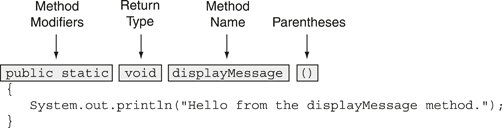
\includegraphics[scale=0.9]{Images/chapter05_methodDescription.png}
    \end{figure}    
\end{frame}

\begin{frame}[fragile]{Calling a Method}
    \vspace{1em} 
    The \textbf{main} method is automatically called when a program starts. \\ 
    \vspace{1em} 
    Other methods are executed by method call statements.
    \begin{lstlisting}
public class SimpleMethod { 
    public static void main(String[] args) {
        System.out.println("Hello from the main method.");
        displayMessage();
        System.out.println("Back in the main method.");
        }
    public static void displayMessage() {
        System.out.println("Hello from the displayMessage method."); 
        }
    }
    \end{lstlisting}
\end{frame}

\begin{frame}[fragile]{Layered Method Calls}
Methods can also be called in layered fashion. \\ 
\vspace{1em}
Method A can call method B, which can then call method C.
\begin{lstlisting}[basicstyle=\ttfamily\scriptsize]
public class DeepAndDeeper {
    public static void main(String[] args) {
        System.out.println("I am starting in main.");
        deep();
        System.out.println("Now I am back in main.");
        }
    public static void deep() {
        System.out.println("I am now in deep.");
        deeper();
        System.out.println("Now I am back in deep.");
        }
    public static void deeper() {
        System.out.println("I am now in deeper.");
        }
    }
\end{lstlisting}
\end{frame}

\section{Method Arguments}
\subsection{Passing Arguments to a Method}
\begin{frame}[fragile]{Passing Arguments to a Method}
A method may be written so it accepts arguments. \\ 
\vspace{1em} 
Data can then be passed into the method when it is called.
\begin{lstlisting}
// The method is println, the argument is the string "Hello".
System.out.println("Hello");
\end{lstlisting}
As another example, consider
\begin{lstlisting}
public static void displayValue(int num) {
    System.out.println("The value is " + num); 
    }
\end{lstlisting}
where the parenthesis enables the method to accept an integer value as an argument.
\end{frame}

\begin{frame}[fragile]{Argument and Parameter Data Type Compatibility}
    Be sure that the argument’s data type is compatible with the parameter variable’s data type. \\
    \vspace{1em}
    Java will perform a widening conversion if the argument’s data type is ranked lower than the parameter variable’s data type. \\ 
    \vspace{1em}
    Java will not automatically convert an argument to a lower-ranking data type (\textbf{long}, \textbf{float}, or \textbf{double} value cannot be passed to a method that has an \textbf{int} parameter).
\begin{lstlisting}
short s = 1;
displayValue(s); // Converts short to int
byte b = 2;
displayValue(b); // Converts byte to int
double d = 1.0;
displayValue(d); // Error! Can’t convert double to int.
\end{lstlisting}
\end{frame}

\begin{frame}[fragile]{Passing Multiple Arguments}
    We can also pass multiple arguments to a method by separating them with a comma.
    \begin{lstlisting}
public static void showSum(double num1, double num2) { 
    double sum;
    sum = num1 + num2;
    System.out.println("The sum is " + sum);
    }
    \end{lstlisting}
\end{frame}

\subsection{Pass by Value and Passing Object References}
\begin{frame}[fragile]{Pass by Value}
\red{Note all primitive data types are passed by value.}
    \begin{lstlisting}
public class PassByValue {
    public static void main(String[] args) {
        int number = 99; // number starts with 99
        System.out.println("number is " + number);
        changeMe(number);
        System.out.println("number is " + number);
        }
    public static void changeMe(int myValue) {
        System.out.println("I am changing the value.");
        myValue = 0;
        System.out.println("Now the value is " + myValue);
            }
        }        
    \end{lstlisting}
\end{frame}

\begin{frame}[fragile]{Passing Object References}
    You can also write methods that accept references to objects as arguments.
    \begin{lstlisting}
public class PassByReference {
    public static void main(String[] args) {
        String name = "Warren";
        showLength(name);
        }
    public static void showLength(String str) {
        System.out.println(
            str 
            + " is " + str.length() 
            + " characters long."); 
        }
    }
    \end{lstlisting}
\end{frame}

\section{Local Variables and Returning Values from a Method}
\subsection{Local Variables}
\begin{frame}{Local Variables}
    A \red{local variable} is declared \red{inside a method} and is not accessible to statements outside the method. \\ 
    \vspace{1em}
    Different methods can have local variables with the same names because the methods cannot see each other’s local variables. \\ 
    \vspace{1em}
    A method’s local variables exist only while the method is executing. \\
    \vspace{1em}
    This is known as the lifetime of a local variable. \\ 
    \vspace{1em}
\end{frame}

\begin{frame}[fragile]{Local Variables}
    \begin{lstlisting}
public static void main(String[] args) {
	texas();
	california();
	}
public static void texas() {
	int birds = 5000;  // variable "birds" in texas method
	System.out.println(
		"In texas there are "
		+ birds + " birds.");
		}
public static void california() {
	int birds = 3500;  // variable "birds" in california method
	System.out.println(
		"In california there are " +
		birds + " birds.");
	}
    \end{lstlisting}
\end{frame}

\subsection{Returning a Value from a Method}
\begin{frame}[fragile]{Returning a Value from a Method}
    You've seen that data may be passed into a method by way of parameter variables. \\ 
    \vspace{1em}
    Data may also be returned from a method, back to the statement that called it. \\ 
    \vspace{1em}
    Methods that return a value are appropriately known as \red{value-returning methods}.
    \begin{lstlisting}
int num;
String someWord = "Hello";
num = someWord.length(); // value-returning method example
    \end{lstlisting}
\end{frame}

\begin{frame}[fragile]{Returning a Value from a Method}
    So how do we \red{define} value-returning methods? \\
    \vspace{1em}
    You must decide what type of value is being returned. \\ 
    \vspace{1em}
    A value-returning method will use \textbf{void, int, double, boolean}, or any other valid data type in its header.
    \begin{lstlisting}
public static int sum(int num1, int num2) { // Returns int
    int result;
    result = num1 + num2;
    return result; // "return" keyword is required
    }
    \end{lstlisting}
\end{frame}

\begin{frame}[fragile]{Returning a Value from a Method}
\begin{lstlisting}[basicstyle=\ttfamily\footnotesize]
public class RangeChecker {
    public static void main(String[] args) {
		int value = 20;
		if (isValid(value))
			System.out.print("The value is within range.");
		else
			System.out.print("The value is out of range.");
		}
	public static boolean isValid(int number) {
		boolean status;
		if (number >= 1 && number <= 100)
			status = true;
		else
			status = false;
		return status;
		}
	}
\end{lstlisting}    
\end{frame}

\subsection{Returning an Object from a Method}
\begin{frame}[fragile]{Returning an Object from a Method}
A value-returning method can also return a reference to a non-primitive data type such as a \textbf{String} object.
\begin{lstlisting}
public class ReturnString {
    public static void main(String[] args) {
        String customerName;
        customerName = fullName("John", "Doe");
        System.out.print(customerName);
        }
    public static String fullName(String first, String last) {
        String name = first + " " + last;
        return name;
        }
    }
\end{lstlisting}
\end{frame}

\subsection{Problem Solving with Methods}
\begin{frame}{Problem Solving with Methods}
See lecture video for a breakdown of the SalesReport.java file.
\end{frame}


% \subsection{Increment and Decrement Operators}
% \begin{frame}{Increment and Decrement Operators}
%     Before getting into loops, we'll briefly cover the \violet{increment (++)} and \violet{decrement (--)} operators. These operators can increase and decrease the value of a variable by one. Both update the value of the operand to its new value. They have two forms: prefix and postfix.
% \end{frame}

\end{document}

